\documentclass[12pt,a4paper]{report}
\usepackage[top=0.75cm,bottom=1.5cm,right=1cm,left=1cm]{geometry}
\usepackage{eso-pic}
\usepackage{amsmath,amsfonts,amssymb,amsthm,mathrsfs,pgfornament}
\usepackage{amssymb}
\usepackage{multicol}
\setlength{\columnseprule}{1pt}

\newcommand{\R}{\mathbb{R}}

\usepackage[most]{tcolorbox}
\pagestyle{empty}
\definecolor{fff}{RGB}{0,139,180}
\definecolor{ggg}{RGB}{8,81,102}
\tikzset{a/.style={anchor=west,line width=1.5pt,font=\bfseries\Large,rounded corners=2mm,draw=white,text=black,inner xsep=5mm,minimum height=1.3cm,rotate=-90}}
\usetikzlibrary{calc}
\usetikzlibrary{shapes.geometric}
\renewcommand{\labelenumi}{%
	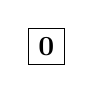
\begin{tikzpicture}[baseline=(1.base)]
	\node[draw,regular polygon,regular polygon sides=4,inner sep=.5mm,fill=white,font=\bfseries](1){\arabic{enumi}};
	\end{tikzpicture}}
\renewcommand{\labelenumii}{%
	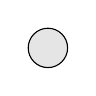
\begin{tikzpicture}[baseline=(1.base)]
	\node[draw,circle,inner sep=.5mm,fill=gray!20,font=\bfseries\footnotesize,minimum size=5mm](1){\alph{enumii}};
	\end{tikzpicture}}





\usepackage{pifont,bbding}
\usepackage{hyperref, tikz}
\usepackage{varwidth}
%\usepackage[object=vectorian]{pgfornament}
%\usetikzlibrary{shapes.multipart}
\newcommand{\circled}[1]{\tikz[baseline=-6pt] 
	\node[circle,draw=gray,inner sep=1.5pt]{#1};} 
\definecolor{yt}{HTML}{c71610}


\DeclareTColorBox{boxe}{ O{black} O{df}}{enhanced,breakable,
	before skip=2mm,after skip=0.3cm,
	bottom=0.5cm,colframe=#1,
	colback=#1!2,boxrule=0.2mm,arc=2mm,drop midday shadow=#1,
	attach boxed title to top left={xshift=0cm,yshift*=0mm-\tcboxedtitleheight},
	varwidth boxed title*=-3cm,
	boxed title style={frame code={
			\path[fill=#1]
			([xshift=+0.5cm]frame.north east)[rounded corners=2mm]--(frame.north west)[sharp corners]--(frame.south west) --(frame.south east)to[out=0,in=180]cycle;
			\draw[#1]([yshift=-0.5mm]frame.south west)--([yshift=-0.5mm,xshift=+0.4mm]frame.south east)to[out=0,in=180]([yshift=0mm,xshift=+0.58cm]frame.north east);
		},interior engine=empty,
	},title={\large\bf #2},pad at break*=4mm}
\begin{document}
	
\begin{center}
		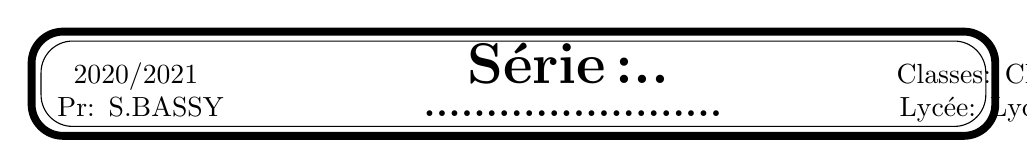
\begin{tikzpicture}
	\node[rectangle,rounded corners=4mm,line width=1mm,align=center,draw,minimum width=\textwidth , text width=0.99\textwidth](1){
		
		
\begin{tabular}{c c  c}
$2020/2021$ 	\hspace*{2cm}   & \textbf{{\huge Série :..   }} & 	\hspace*{1.5cm} Classes: Classe 1 Classe			\\
Pr: S.BASSY\hspace*{2cm} &{\Large \textbf{ ........................ }} & \hspace*{1cm}Lycée: Lycée Lycée
\end{tabular}


};
	\draw[rounded corners=4mm]([xshift=1.7mm,yshift=-1.7mm]1.north west)
	rectangle([xshift=-1.7mm,yshift=1.7mm]1.south east);
	\end{tikzpicture}
\end{center}

%\begin{multicols}{2}
	\begin{boxe}[black][Exercice $1$]
	
	\begin{enumerate}
		\item Déterminer 
		\item On pose.\begin{enumerate}
			\item Déterminer 
			\item Montrer 
			\item En déduire 
			
		\end{enumerate}
		
	\end{enumerate}
	\end{boxe}

		\begin{boxe}[black][Exercice $2$]
		
		\begin{enumerate}
			\item Déterminer 
			\item On pose.\begin{enumerate}
				\item Déterminer 
				\item Montrer 
				\item En déduire 
				
			\end{enumerate}
			
		\end{enumerate}
	\end{boxe}
	
	
	\begin{boxe}[black][Exercice $3$]
	
	\begin{enumerate}
		\item Déterminer 
		\item On pose.\begin{enumerate}
			\item Déterminer 
			\item Montrer 
			\item En déduire 
			
		\end{enumerate}
		
	\end{enumerate}
\end{boxe}
	
	
	

	\begin{boxe}[black][Exercice $4$]
	
	\begin{enumerate}
		\item Déterminer 
		\item On pose.\begin{enumerate}
			\item Déterminer 
			\item Montrer 
			\item En déduire 
			\item Montrer 
		\end{enumerate}
		\item On pose.
		\begin{enumerate}
			\item Déterminer 
			\item Montrer 
			\item En déduire 
			\item Montrer 
		\end{enumerate}
	\end{enumerate}
\end{boxe}

\begin{boxe}[black][Exercice $4$]
	
	\begin{enumerate}
		\item Déterminer 
		\item On pose.\begin{enumerate}
			\item Déterminer 
			\item Montrer 
			\item En déduire 
			\item Montrer 
		\end{enumerate}
		\item On pose.
		\begin{enumerate}
			\item Déterminer 
			\item Montrer 
			\item En déduire 
			\item Montrer 
		\end{enumerate}
	\end{enumerate}
\end{boxe}










\end{document}